\documentclass{beamer}
\usepackage{tikz,amsmath,hyperref,graphicx,stackrel,animate,setspace}
\usetikzlibrary{positioning,shadows,arrows,shapes,calc}
\newcommand{\argmax}{\operatornamewithlimits{argmax}}
\newcommand{\argmin}{\operatornamewithlimits{argmin}}
\mode<presentation>{\usetheme{Frankfurt}}
\DeclareMathOperator*{\softmax}{softmax}
\AtBeginSection[]
{
  \begin{frame}<beamer>
    \frametitle{Outline}
    \tableofcontents[currentsection,currentsubsection]
  \end{frame}
}
\title{Lecture 21: Faster RCNN}
\author{Mark Hasegawa-Johnson\\All content~\href{https://creativecommons.org/licenses/by-sa/4.0/}{CC-SA 4.0} unless otherwise specified.}
\date{ECE 417: Multimedia Signal Processing, Fall 2021}  
\begin{document}

% Title
\begin{frame}
  \maketitle
\end{frame}

% Title
\begin{frame}
  \tableofcontents
\end{frame}


%%%%%%%%%%%%%%%%%%%%%%%%%%%%%%%%%%%%%%%%%%%%
\section[Review]{Review: Neural Network}
\setcounter{subsection}{1}

\begin{frame}
  \frametitle{Review: How to train a neural network}
  \begin{enumerate}
  \item Find a {\bf training dataset} that contains $n$ examples showing the
    desired output, $\vec{y}_i$, that the NN should compute in
    response to input vector $\vec{x}_i$:
    \[
    {\mathcal D}=\left\{(\vec{x}_1,\vec{y}_1),\ldots,(\vec{x}_n,\vec{y}_n)\right\}
    \]
    \item Randomly {\bf initialize} the weights and biases, $W^{(1)}$,
      $\vec{b}^{(1)}$, $W^{(2)}$, and $\vec{b}^{(2)}$.
    \item Perform {\bf forward propagation}: find out what the neural
      net computes as $\hat{y}_i$ for each $\vec{x}_i$.
    \item Define a {\bf loss function} that measures
      how badly $\hat{y}$ differs from $\vec{y}$.
    \item Perform {\bf back propagation} to improve $W^{(1)}$,
      $\vec{b}^{(1)}$, $W^{(2)}$, and $\vec{b}^{(2)}$.
    \item Repeat steps 3-5 until convergence.
  \end{enumerate}
\end{frame}

\begin{frame}
  \frametitle{Review: Fully-connected and Convolutional Neural Networks}
  \begin{itemize}
  \item Fully-connected layers: forward-prop is a matrix multiplication, back-prop
    is multiplication by the transposed matrix, weight gradient is a vector outer product.
  \item Convolutional layers: forward-prop is a convolution, back-prop
    is a correlation, weight gradient is a convolution.
  \item Max pooling: back-prop just propagates the derivative to the
    pixel that was chosen by forward-prop.
  \end{itemize}
\end{frame}

\begin{frame}
  \frametitle{Error Metrics Summarized}
  \begin{itemize}
    \item Use MSE to achieve $\hat{y}\rightarrow
      E\left[\vec{y}|\vec{x}\right]$.  That's almost always what you
      want.
    \item For a binary classifier with a sigmoid output, BCE loss gives you
      the MSE result without the vanishing gradient problem.
    \item For a multi-class classifier with a softmax output, CE loss gives you
      the MSE result without the vanishing gradient problem.
    \item After you're done training, you can make your cell phone app
      more efficient by throwing away the uncertainty:
      \begin{itemize}
      \item Replace softmax output nodes with max
      \item Replace logistic output nodes with unit-step
      \item Replace tanh output nodes with signum
      \end{itemize}
  \end{itemize}
\end{frame}

%%%%%%%%%%%%%%%%%%%%%%%%%%%%%%%%%%%%%%%%%%%%
\section{Object Detection}
\setcounter{subsection}{1}

\begin{frame}
  \frametitle{Object Recognition vs. Object Detection}
  \begin{itemize}
  \item {\bf Object Recognition}
    \begin{itemize}
    \item The task: Decide which objects are present in an image.
    \item SOTA solution: very deep convolutional neural nets.
    \end{itemize}
  \item {\bf Object Detection}
    \begin{itemize}
    \item The task: Figure out where the object is in the image.
    \item SOTA solution: RPN w.r.t. anchors fixed w.r.t. ROI.
    \end{itemize}
  \end{itemize}
\end{frame}

\begin{frame}
  \frametitle{Object Detection Example}
  \begin{columns}
    \column{2in}
    \begin{block}{WIDER FACE Dataset (Yang, Luo, Loy \& Tang, 2016)}
      \begin{itemize}
      \item Dataset published 2015 w/13k images, 300k+ faces.
      \item Bounding box for each face given as (x,y,w,h).
      \item Metadata: blur, expression, illumination, occlusion, pose.
      \item In the example at right, I've eliminated all faces with
        nonzero blur, illumination, or occlusion.
      \end{itemize}
    \end{block}
    \column{2.5in}
    \begin{block}{}
      \centerline{\includegraphics[width=2.45in]{exp/mp3_ref.png}}
    \end{block}
  \end{columns}
\end{frame}

\begin{frame}
  \frametitle{Object Detection as Classification}
  
  Suppose that we are given a region of interest, $ROI=(x,y,w,h)$, and
  asked to decide whether the ROI is an object.  We can do this by
  training a neural network to estimate the classifier output:
  \[
  y_c(ROI) = \begin{cases}
    1 & \mbox{ROI contains an object}\\
    0 & \mbox{ROI does not contain  an object}
  \end{cases}
  \]
  A neural net trained with MSE or CE will then compute
  \[
  \hat{y}_c=\Pr\left(\mbox{ROI contains an object}\right)
  \]
\end{frame}

\begin{frame}
  \frametitle{Training a network for object detection}
  
  Back-prop to the individual pixels can show the degree to which each
  pixel contributes to the detection probability.  Here's an example
  based on Gaussian supervectors (Zhuang et al., ``Efficient Object
  Localization with Gaussianized Vector Representation,'' 2009):
  \centerline{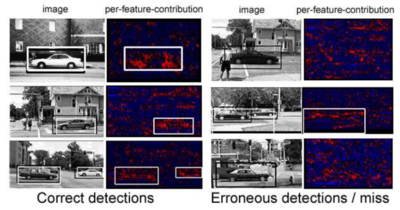
\includegraphics[height=2in]{figs/zhuang2009_fig4.png}}
  
\end{frame}

\begin{frame}
  \frametitle{What about partial overlap?}

  Real networks need to deal with situations of partial overlap, e.g., 
  \centerline{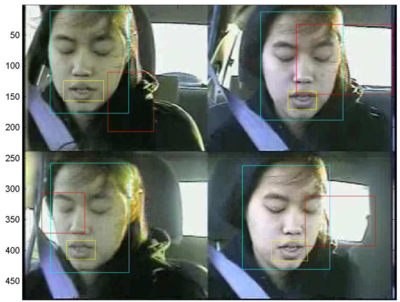
\includegraphics[height=2.25in]{figs/avicar_rects.png}}
  \begin{tiny}Lee, Hasegawa-Johnson, Goudeseune, Kamdar, Borys, Liu \& Huang (2004)\end{tiny}
\end{frame}


\begin{frame}
  \frametitle{Intersection  over union (IOU)}
  
  We deal with partial-overlap by putting some sort of threshold on
  the intersection-over-union measure.  Suppose the hypothesis is
  $(x_{ROI},y_{ROI},w_{ROI},h_{ROI})$, and the reference is
  $(x_{REF},y_{REF},w_{REF},h_{REF})$, then IOU is
  \begin{displaymath}
    IOU =\frac{I}{U}=
    \frac{\mbox{number of pixels in both ROI and REF}}{\mbox{number of pixels in either ROI or REF}},
  \end{displaymath}
  where the intersection between REF  and ROI is:
  \begin{align*}
    I &= \left(\min\left(x_{REF}+w_{REF},x_{ROI}+w_{ROI}\right)-\max\left(x_{REF},x_{ROI}\right)\right)
    \times\\
    &\left(\min\left(y_{REF}+h_{REF},y_{ROI}+h_{ROI}\right)-\max\left(y_{REF},y_{ROI}\right)\right),
  \end{align*}
  and their union is:
  \begin{displaymath}
    U = w_{REF}h_{REF}+w_{ROI}h_{ROI}-I
  \end{displaymath}
\end{frame}

\begin{frame}
  \frametitle{Arbitrary  Thresholds on IOU}
  
  We could use IOU as a soft-measure, or could we put some sort of
  arbitrary threshold, like:
  \[
  y_c(ROI) = \begin{cases}
    1 & IOU>0.7\\
    0 & \mbox{otherwise}
  \end{cases}
  \]
  Then we get:
  \[
  \hat{y}_c=\Pr\left(IOU > 0.7\right)
  \]
\end{frame}

\begin{frame}
  \frametitle{Training a network for object detection}
  
  Here is one of the MP3 object detectors:
  
  \centerline{\includegraphics[height=2.15in]{exp/mp3_ref.png}\includegraphics[height=2.15in]{exp/anchor0prob.png}}
  
\end{frame}


%%%%%%%%%%%%%%%%%%%%%%%%%%%%%%%%%%%%%%%%%%%%%%%%%%%%%%%%%%%%%%%%%%%%%%%%%%%%%%%%%%%%%%
\section[ROI]{Regions of Interest}
\setcounter{subsection}{1}

\begin{frame}
  \frametitle{Why Object Detection is Hard: Too Many Rectangles}
  \begin{itemize}
  \item Suppose the image is $N\times N$, e.g., $N\approx 1000$.
  \item A bounding-box rectangle is $(x,y,w,h)$, so there are
    $O\left\{N^4\right\}\approx 10^{12}$ rectangles to evaluate.
  \item If it takes the classifier $100\mu s$ to evalute one
    rectangle, then it takes $10^8$ seconds = 3.17 years to evaluate
    all of the rectangles in an image.
  \end{itemize}
\end{frame}

\begin{frame}
  \frametitle{Object Detection: Solutions}
  \begin{enumerate}
  \item Very fast classifiers: e.g., Viola-Jones Adaboost.
  \item Region proposal network (RPN): category-independent object
    proposals.
  \item Fast RCNN: RPN computed as a nonlinear regression, w.r.t. a
    predefined ROI.
  \item Faster-RCNN: RPN computed as a nonlinear regression, w.r.t. a
    predefined anchor, which is defined w.r.t. a predefined ROI.
  \end{enumerate}
\end{frame}


\begin{frame}
  \begin{columns}
    \column{2.25in}
    \begin{block}{Solution \#1: Very Fast Classifiers}
      \centerline{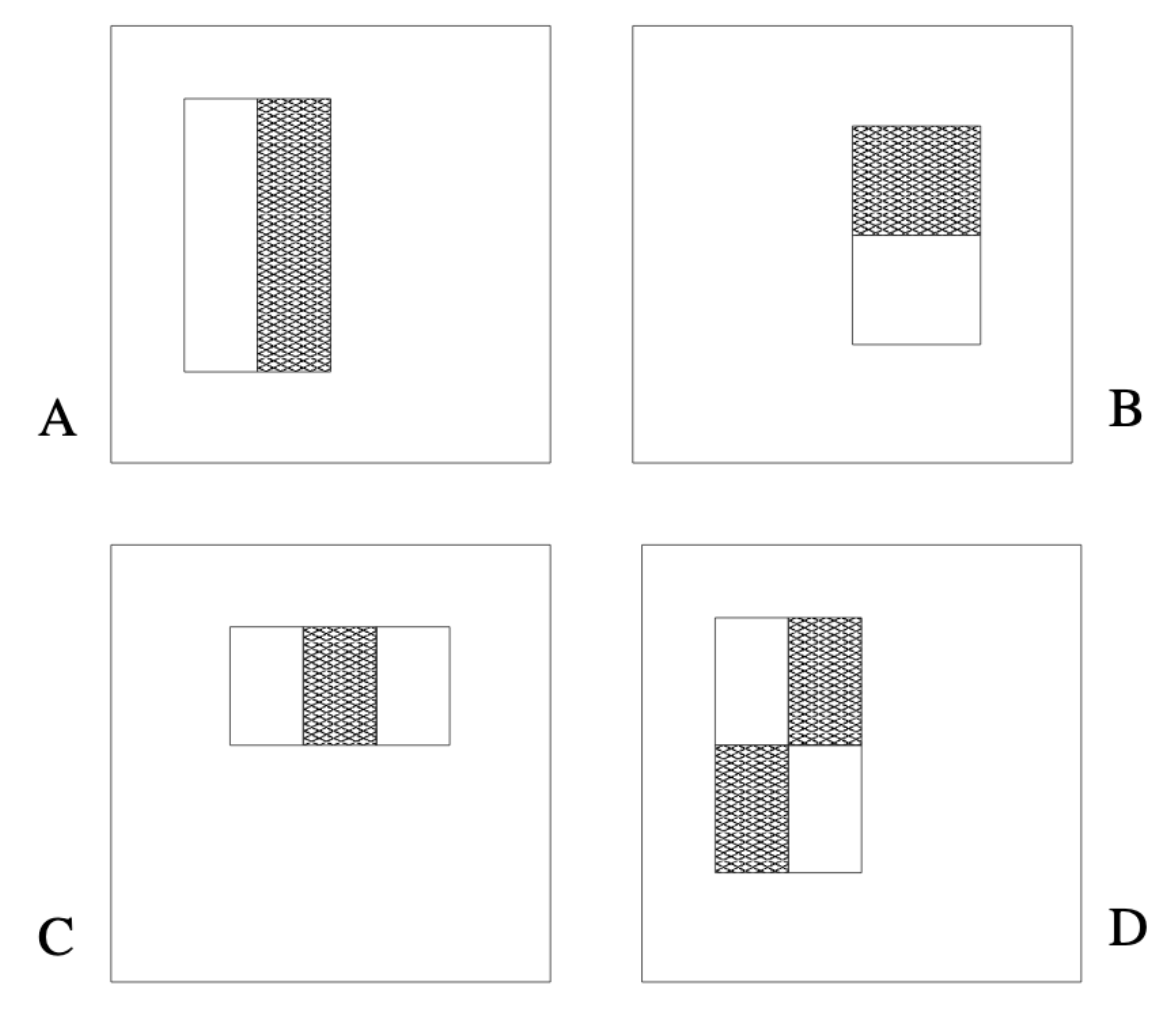
\includegraphics[width=2.15in]{figs/violajones_fig1.png}}
      \begin{tiny}Image copyright Viola \& Jones, 2001\end{tiny}
    \end{block}
    \column{2.25in}
    \begin{block}{``Rapid Object Detection using a Boosted Cascade of Simple Features,'' Viola and Jones, 2001}
      \begin{itemize}
      \item Each weak classifier evaluates just one Haar feature
        (features shown at left), which can be computed using only
        $\sim 6$ additions/rectangle.
      \item Most rectangles eliminated after a cascade of just two
        weak classifiers (so: nanoseconds, not microseconds).
      \end{itemize}
    \end{block}
  \end{columns}
\end{frame}

\begin{frame}
  \frametitle{Solution \#2: ``Category-Independent Object Proposals,'' Endres \& Hoiem, 2010}
  \centerline{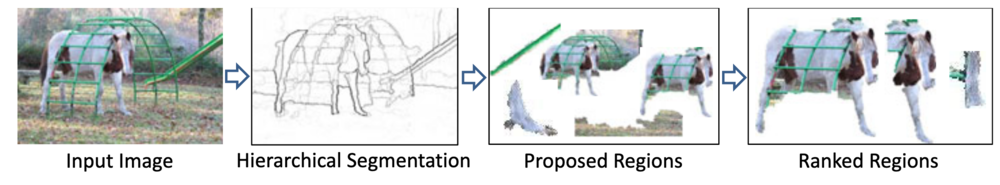
\includegraphics[width=4.5in]{figs/endres_hoiem_fig1.png}}
  \begin{tiny}Image copyright Endres \& Hoiem, 2010\end{tiny}
  \begin{itemize}
  \item Pixels accumulated into candidate regions-of-interest
    (ROI) based on similarity of texture, color, etc.
  \item Candidate ROIs ranked by a neural net.
  \item Neural net trained to decide whether an ROI contains a
    nameable object or not, regardless of what type of object it
    is.
  \end{itemize}
\end{frame}

\begin{frame}
  \frametitle{Solution \#3: ``Fast RCNN,'' Girshick, 2015}
  \centerline{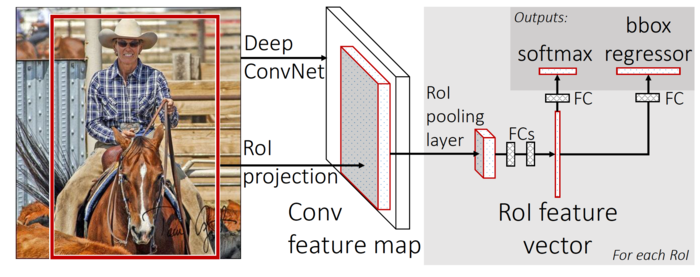
\includegraphics[height=1.5in]{figs/girshick2015_fig1.png}}
  \begin{tiny}Image copyright Girshick, 2015\end{tiny}
  \begin{itemize}
  \item Start with a small set of candidate ROIs (a few hundred
    per image)
  \item Each ROI feeds a neural net whose output is a 4-vector
    specifying the (x,y,w,h) of the nearest object.
  \end{itemize}
\end{frame}

\begin{frame}
  \frametitle{ROI: Variable vs. Fixed}
  \begin{itemize}
  \item Previous object detectors, up through RCNN, computed ROI
    candidates in a bottom-up fashion, so that different images would
    have different ROI candidates.
  \item Fast RCNN proposed using fixed ROI candidates, that are exactly the
    same in every image.
    \begin{itemize}
    \item That way, you don't have to waste time figuring out where the ROIs are.
    \item Girchick's proposal: just use 
      the last convolutional layer of an object recognizer like VGG16.
    \end{itemize}
  \end{itemize}
\end{frame}

\begin{frame}
  \frametitle{VGG16: ``Very Deep Convolutional Networks for Large-Scale Image Classification''}
  \centerline{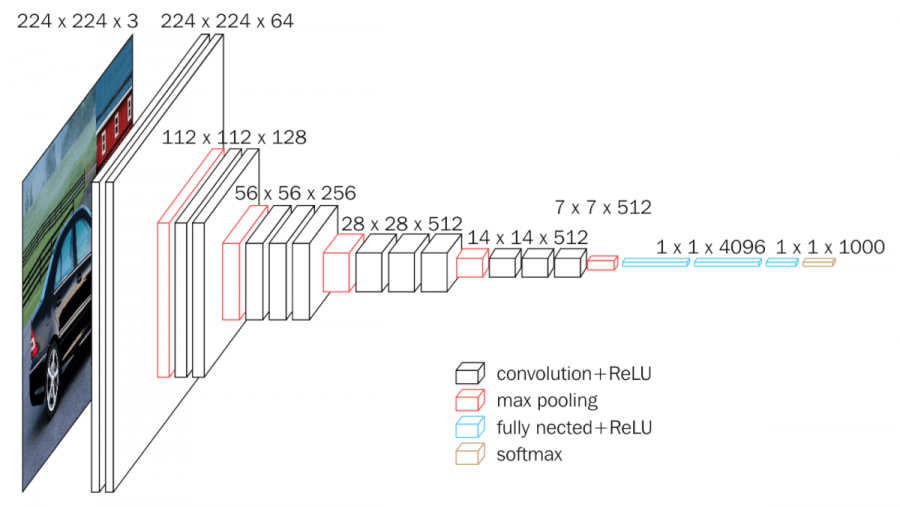
\includegraphics[height=1.5in]{figs/vgg16.png}}
  \begin{tiny}Image copyright Simonyan \& Zisserman, 2015\end{tiny}  
  \begin{itemize}
  \item Input normalized to $224\times 224$ pixels, 3 color channels.
  \item Last convolutional layer is $14\times 14$ pixels, 512 channels.  Call this
    $\vec{f}[m,n]$, where $\vec{f}\in\Re^{512}$, $0\le (m,n)\le 13$.
  \item Output FCN trained for object recognition: 1000 different object types.
  \end{itemize}
\end{frame}


%\begin{frame}
%  \frametitle{Using VGG16 as ROI Features for RPN}
%  \begin{itemize}
%  \item Faster RCNN assumes that the original image is $1064\times
%    1064$ pixels, which is then downsampled to the $224\times
%    224$-pixel size required as input to VGG16.
%  \item There are 4 layers of max pooling before the last conv layer,
%    so each feature vector in the last conv layer represents
%    \[
%    \left(2^4\left(\frac{1064}{224}\right)\right)\times\left(2^4\left(\frac{1064}{224}\right)\right)=
%    76\times 76~\frac{\mbox{input pixels}}{\mbox{feature vector}}.
%    \]
%  \item The last conv layer contains
%    \[
%    \left(\frac{224}{2^4}\right)\times\left(\frac{224}{2^4}\right)=14\times
%    14=196~\mbox{feature vectors}.
%    \]
%  \end{itemize}
%\end{frame}

\begin{frame}
  \frametitle{Last conv layer contains $14\times 14=196$ ROIs}
  \centerline{\includegraphics[height=3in]{exp/grid14x14.png}}
\end{frame}


\begin{frame}
  \begin{columns}
    \column{2.25in}
    \begin{block}{ROI = $3\times 3$ grid of VGG16 feature vectors}
      \centerline{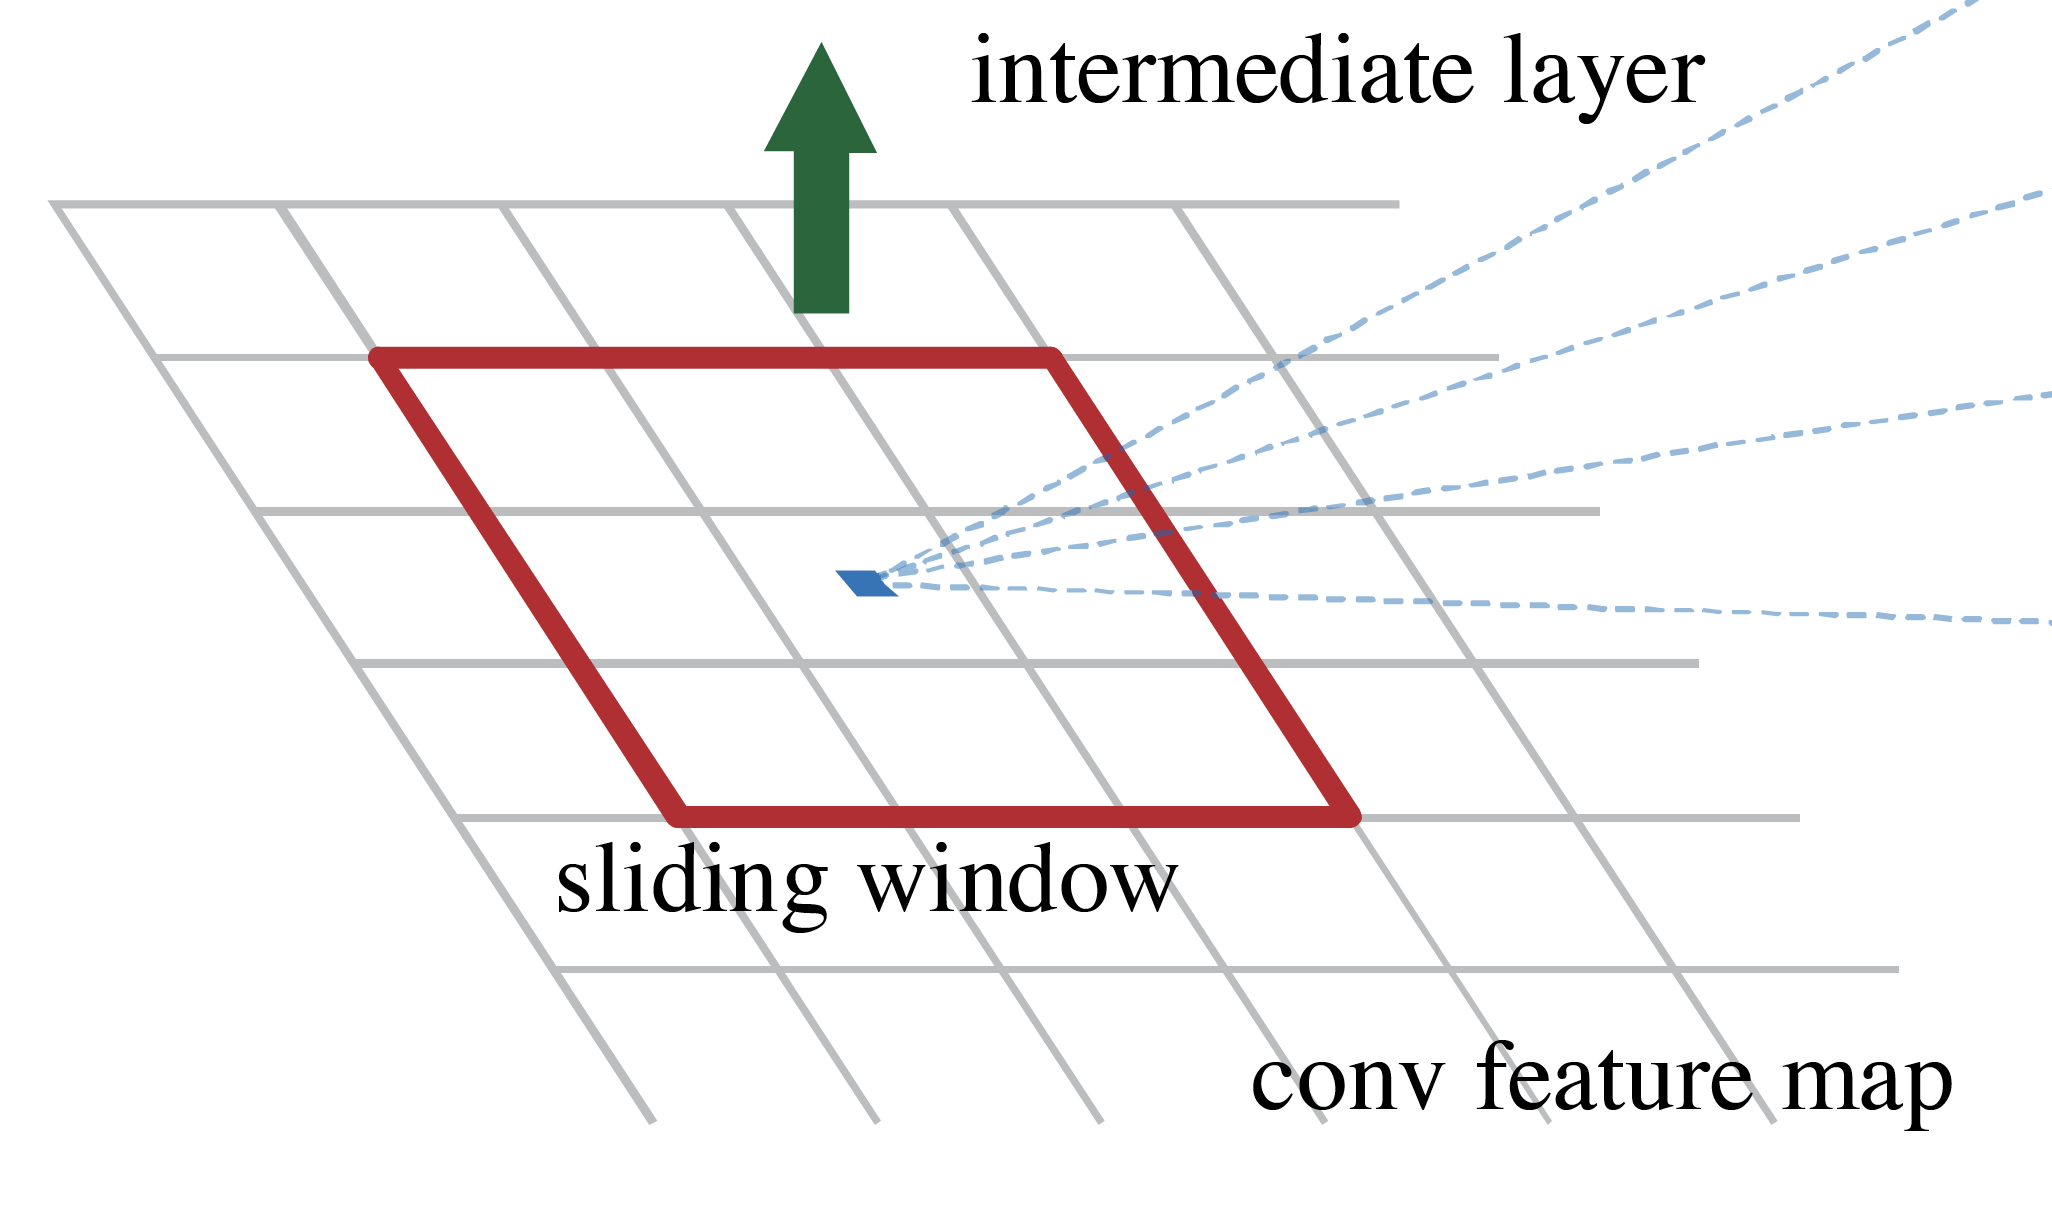
\includegraphics[width=2.15in]{figs/ren2016fig2a.png}}
      \begin{tiny}Image copyright Ren, He, Girshick \& Sun, 2016\end{tiny}
    \end{block}
    \column{2.25in}
    \begin{block}{}
      The region proposal network takes, as input, the concatenation
      of nine neighboring feature vectors from the VGG16 layer:
      \[
      \vec{x}_{m,n}=\left[\begin{array}{c}
          \vec{f}[m-1,n-1]\\
          \vec{f}[m-1,n]\\
          \vdots\\
          \vec{f}[m+1,n+1]
        \end{array}\right]
      \]
      Notice, we could think of this as another convolutional layer,
      but Fast RCNN just treats it as a fully-connected network.
    \end{block}
  \end{columns}
\end{frame}

\begin{frame}
  \frametitle{ROI = $3\times 3$ grid of VGG16 feature vectors}
  \centerline{\includegraphics[height=2.5in]{exp/concatenated_features.png}}
      \[\vec{x}_{m,n}=[\vec{f}[m-1,n-1],\vec{f}[m-1,n],\ldots,\vec{f}[m+1,n+1]]\]
\end{frame}


%%%%%%%%%%%%%%%%%%%%%%%%%%%%%%%%%%%%%%%%%%%%%%%%%%%%%%%%%%%%%%%%%%%%%%%%%%%%%%%%%%%%%%
\section[Regression]{Bounding Box Regression}
\setcounter{subsection}{1}

\begin{frame}
  \frametitle{What pixels are covered by the ROI called
    $\vec{f}_{m,n}$?}

  The $(m,n)^{\textrm{th}}$ feature vector, $\vec{f}_{m,n}$, covers a
  particular block of pixels in the input image:
  \[
  (x_{ROI},y_{ROI},w_{ROI},h_{ROI}) =
  (76n, 76m, 228,228)
  \]
  \begin{itemize}
  \item Each $\vec{x}[m,n]$ covers $76\times 76$ input pixels.
  \item Each $\vec{f}_{m,n}$ is $(3\cdot 76)\times(3\cdot 76)=228\times 228$.
  \item $m\rightarrow y$ is the vertical axis, $n\rightarrow x$ horizontal.
  \end{itemize}
\end{frame}

\begin{frame}
  \frametitle{What pixels {\bf\em should} be covered?}

  Suppose the nearest true object is in rectangle
  $(x_{REF},y_{REF},w_{REF},h_{REF})$.  We want to somehow encode the
  difference between where we are now
  ($x_{ROI},y_{ROI},w_{ROI},h_{ROI}$) and where we want to be
  ($x_{REF},y_{REF},w_{REF},h_{REF}$).  Fast RCNN does this using the
  following target vector, $\vec{y}_r$, for the neural network:
  \[
  \vec{y}_r = \left[\begin{array}{c}
      \frac{x_{REF}-x_{ROI}}{w_{ROI}}\\
      \frac{y_{REF}-y_{ROI}}{h_{ROI}}\\
      \ln\left(\frac{w_{REF}}{w_{ROI}}\right)\\
      \ln\left(\frac{h_{REF}}{h_{ROI}}\right)
    \end{array}\right]
  \]
  The neural net is trained to find a $\hat{y}_r$ that is as close as
  possible to $\vec{y}_r$ (minimum MSE).
\end{frame}


\begin{frame}
  \frametitle{Training a bbox regression network}

  The network is now trained with two different outputs, $\hat{y}_c$
  and $\hat{y}_r$.  The total loss is
  \begin{displaymath}
    {\mathcal L}={\mathcal L}_c+{\mathcal L}_r
  \end{displaymath}
  where ${\mathcal L}_c$ is BCE for the classifier output:
  \begin{displaymath}
    {\mathcal L}_c = -\frac{1}{n}\sum_{i=1}^n \left(y_{c,i}\ln\hat{y}_{c,i}+(1-y_{c,i})\ln(1-\hat{y}_{c,i})
    \right)
  \end{displaymath}
  and ${\mathcal L}_r$ is zero if $y_c=0$ (no object present), and MSE
  if $y_c=1$:
  \begin{displaymath}
    {\mathcal L}_r = \frac{1}{2}
    \frac{\sum_{i=1}^n y_{c,i}\Vert\vec{y}_{r,i}-\hat{y}_{r,i}\Vert^2}{\sum_{i=1}^n y_{c,i}}
  \end{displaymath}
\end{frame}
    
%%%%%%%%%%%%%%%%%%%%%%%%%%%%%%%%%%%%%%%%%%%%%%%%%%%%%%%%%%%%%%%%%%%%%%%%%%%%%%%%%%%%%%
\section[Anchors]{Fixed Anchor Rectangles}
\setcounter{subsection}{1}

\begin{frame}
  \begin{columns}
    \column{2.25in}
    \begin{block}{``Faster R-CNN: Towards Real-Time Object
        Detection with Region Proposal Networks,'' Ren, He, Girshick \& Sun,
        2016}
      \centerline{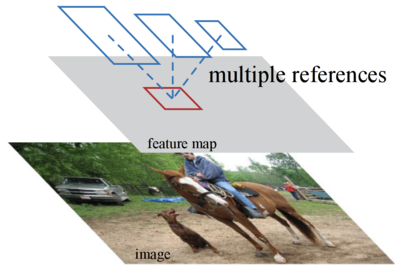
\includegraphics[width=2.15in]{figs/ren2016_fig1c.png}}
      \begin{tiny}Image copyright Ren, He, Girchick \& Sun, 2016\end{tiny}      
    \end{block}
    \column{2.25in}
    \begin{block}{}
      \begin{itemize}
      \item Each candidate bounding box computes 9 different
        regression outputs, each of which is a 4-vector (x,y,w,h)
      \item The 9 different regression outputs from each bbox are
        w.r.t. 9 different ``anchor'' rectangles, each offset from the
        input ROI.  Thus:
        \begin{align*}
          \mbox{anchor} &= \mbox{ROI}+ \mbox{known shift}\\
          \mbox{object} &= \mbox{anchor}+ \mbox{regression}
        \end{align*}
      \end{itemize}
    \end{block}
  \end{columns}
\end{frame}


\begin{frame}
  \frametitle{What pixels {\bf\em should} be covered?}

  \begin{itemize}
  \item The ROI is $(x_{ROI},y_{ROI},w_{ROI},h_{ROI})$.
  \item The anchor is $(x_{a},y_{a},w_{a},h_{a})$.
  \item The true object is located at $(x_{REF},y_{REF},w_{REF},h_{REF})$.
  \item The regression  target is:
    \[
    \vec{y}_r = \left[\begin{array}{c}
        \frac{x_{REF}-x_{a}}{w_{a}}\\
        \frac{y_{REF}-y_{a}}{h_{a}}\\
        \ln\left(\frac{w_{REF}}{w_{a}}\right)\\
        \ln\left(\frac{h_{REF}}{h_{a}}\right)
      \end{array}\right]
    \]
  \end{itemize}
\end{frame}

\begin{frame}
  \begin{columns}
    \column{1.75in}
    \begin{block}{3 sizes, 3 aspect ratios}
      The Faster RCNN paper described 9 anchors per ROI:
      \begin{itemize}
      \item 3 different anchor sizes: $128\times 128$, $256\times
        256$, and $512\times 512$.
      \item 3 different aspect ratios: $1:2$, $1:1$, and $2:1$
      \end{itemize}
    \end{block}
    \column{2.75in}
    \begin{block}{9 anchors per ROI}
      \centerline{\includegraphics[width=2.7in]{exp/anchors.png}}
    \end{block}
  \end{columns}
\end{frame}

%%%%%%%%%%%%%%%%%%%%%%%%%%%%%%%%%%%%%%%%%%%%%%%%%%%%%%%%%%%%%%%%%%%%%%%%%%%%%%%%%%%%%%
\section{Summary}
\setcounter{subsection}{1}

\begin{frame}
  \frametitle{Summary}
  \begin{itemize}
  \item An ROI network has a 4608d input, corresponding to a $3\times
    3$ grid of 512d feature vectors from the last conv layer of a
    VGG16 object recognizer.
  \item Faster-RCNN defines 9 different anchors centered on each ROI.
  \item W.r.t. each anchor, we define the classification target
    $y_c=1$ if $IOU>0.7$, otherwise $y_c=0$.
  \item If $y_c=1$, then we define a regression target $\vec{y}_r$,
    specifying how much the REF bbox differs from the anchor.
  \end{itemize}
\end{frame}
   

\end{document}

